% !TeX root = RJwrapper.tex
\title{GeoThinneR: An R Package for Efficient Spatial Thinning of Species Occurrences and Point Data}


\author{by Jorge Mestre-Tomás}

\maketitle

\abstract{%
In this paper we present GeoThinneR, an R package for efficient and flexible spatial thinning of species occurrence data. Spatial thinning is a widely used preprocessing step in species distribution modeling (SDM) that can help reduce sampling bias, but existing R implementations rely on brute-force algorithms that scale poorly with large datasets. GeoThinneR implements multiple thinning approaches, including ensuring a minimum distance between points, subsampling points on a grid, and filtering based on decimal precision. To handle large datasets, it introduces two optimized algorithms based on local kd-trees and adaptive neighbor estimation, which greatly reduce memory usage and execution time. Additional functionalities such as group-wise thinning and point prioritization are included to facilitate its use in SDM workflows. Here, we provide performance benchmarks using both simulated and real-world data to demonstrate substantial performance improvements over existing tools.
}

\section{Introduction}\label{introduction}

Presence-only data are often the main source of information for modelling species distributions, as systematic survey data are rarely available \citep{pearce2006modelling}. In recent years the availability of spatial biodiversity data has increased, with repositories such as the Global Biodiversity Information Facility (GBIF, \url{https://www.gbif.org}) and the Ocean Biodiversity Information System (OBIS, \url{https://obis.org/}) providing datasets containing hundreds of thousands of species occurrence records. These larger datasets provide new opportunities in ecological research and species distribution modeling (SDM), which are used to model the species geographic distributions based on occurrence records and environmental variables \citep{pulliam2000relationship, elith2009species, miller2010species, guisan2013predicting}. However, as dataset sizes grow, the computational requirements for processing and filtering them increase too. Species occurrence data often show spatial sampling bias due to opportunistic observations, uneven sampling effort or a combination of information from diverse sources that vary in how and where data were collected resulting in heterogeneous datasets \citep{boakes2010distorted, lobo2011exploring, beck2014spatial, meyer2016range, hughes2021sampling}. These biases result in clusters of records that can artificially increase spatial autocorrelation among occurrences and cause the model to overfit the environmental conditions in these oversampled regions, leading to models that reflect patterns in sampling effort rather than true species distributions \citep{wisz2008effects, phillips2009sample, higa2015mapping, cosentino2021geographic, steen2021spatial}.

Several approaches exist to address sampling bias \citep{inman2021comparing, baker2024effective, moudry2024optimising}, including adjusting background points \citep{barber2022target, vollering2019bunching}, applying environmental filtering \citep{castellanos2019environmental}, or incorporating bias-related covariates \citep{varela2014environmental, chauvier2021novel}. Some modelling frameworks attempt to account for sampling bias directly, for example by modelling preferential sampling through point processes \citep{diggle2010geostatistical, pennino2019accounting, amaral2024model} or by combining opportunistically collected presence-only data with systematically sampled data within integrated SDMs \citep{koshkina2017integrated, simmonds2020more, makinen2024integrated}. Here we focus on one of the most widely used preprocessing methods to mitigate these biases across the geographic space, known as spatial thinning, which selectively filters points based on specified criteria to reduce the overrepresentation of the densest locations \citep{veloz2009spatially, boria2014spatial}. The two most common thinning methods in SDM are distance-based thinning, where points are removed if they fall within a specified minimum distance of another point \citep{aiello2015spthin}, and grid-based thinning, which retains only a specified number of points per grid cell \citep{dismoRpackage}.

While existing distance-based thinning tools in R, such as \CRANpkg{spThin} \citep{aiello2015spthin} and \CRANpkg{enmSdmX} \citep{smith2023including}, are widely used, they have several limitations that become more challenging as dataset sizes continue to increase. These tools rely on brute force algorithms for nearest-neighbor searches given a distance threshold, which are unfeasible to run on personal computers as they scale poorly for datasets containing hundreds of thousands of points. On the other hand, grid-based thinning, such as the one implemented in the \CRANpkg{dismo} package \citep{dismoRpackage}, offers better computational efficiency but lacks precision when requiring a specified distance threshold. Additionally, these tools have limited functionality and usability as they often focus on a single thinning approach and offer few customization options for specific SDM applications, such as thinning occurrences across multiple species \citep{noori2024window}. This can be useful when modelling several species or community-level patterns, for example in stacked SDMs (SSDMs) where species are modelled independently and then combined \citep{calabrese2014stacking}, or in joint species distribution models (JSDMs) where multiple species are analysed simultaneously accounting for the multivariate nature of the data \citep{pollock2014understanding, ovaskainen2017make, ovaskainen2020joint}. Other useful features include retaining an exact number of occurrences \citep{steen2021spatial} and prioritizing points based on data quality or other features \citep{yu2023future}.

To overcome these challenges, we introduce \CRANpkg{GeoThinneR} \citep{geothinner2025}, an R package designed to provide efficient and flexible spatial thinning for large-scale datasets. \CRANpkg{GeoThinneR} integrates multiple thinning approaches into a single package simplifying user experience (distance, grid, and decimal precision-based thinning), offers an optimized distance-based thinning using enhanced algorithms based on \emph{kd}-tree structures, which improve nearest-neighbor search efficiency \citep{friedman1975algorithm}, together with additional specific functionalities for SDM workflows including thinning by species or groups, the ability to retain an exact number of occurrences, and prioritization of points based on user-defined variables.

In Section~\hyperref[packagedescription]{2}, we present the methods and features implemented in \CRANpkg{GeoThinneR}. Section~\hyperref[modifiedthinning]{3} contains information about the optimized algorithms for large datasets together with a performance comparison between the distance-based methods available. Section~\hyperref[performancethinning]{4} benchmarks the performance of the package with existing software, both with simulated and real-world datasets. Finally, Section~\hyperref[conclusions]{5} presents a short conclusion of the work and discusses future directions.

\section{GeoThinneR package description}\label{packagedescription}

Given a set of points \(\mathbf{S} = \{ \mathbf{x}_1, \mathbf{x}_2, \dots, \mathbf{x}_n \}\), spatial thinning aims to filter \(\mathbf{S}\) to obtain a subset \(\mathbf{S}' \subseteq \mathbf{S}\) that meets a specified selection criteria. Different thinning methods can be employed to apply this criteria, such as enforcing a minimum separation distance between retained points, limiting the number of points per grid cell, or rounding coordinates to a specified precision. The thinning process iteratively evaluates each point, referred to as the query point \(q\), identifies neighbor points within \(\mathbf{S}\), and applies the selection criteria to return a thinned subset \(\mathbf{S}'\).

The \CRANpkg{GeoThinneR} package is implemented in R and can be downloaded from the Comprehensive R Archive Network (CRAN) at \url{https://cran.r-project.org/package=GeoThinneR}. Comprehensive documentation and usage examples are available on GitHub and CRAN. One of the advantages of \CRANpkg{GeoThinneR} is its flexibility and ease of use, allowing users to efficiently apply different spatial thinning configurations to their datasets. In this section, we demonstrate how to use the package and explore its various thinning methods and additional functionalities.

The main function to apply spatial thinning is \texttt{thin\_points()} which takes a data frame containing a set of points with longitude and latitude columns. The key arguments are the thinning \texttt{method} (\texttt{"distance"}, \texttt{"grid"}, or \texttt{"precision"}), the thinning criterion (\texttt{thin\_dist}, \texttt{resolution}, or \texttt{precision}) and the number of independent thinning attempts (\texttt{trials}). By default, only the subset retaining the largest number of points is returned; to keep all thinning trials, the argument \texttt{all\_trials\ =\ TRUE} must be specified. To illustrate the basic usage, we simulate a toy dataset of 100 uniformly distributed points for two species across an area of 1 x 1 degree and apply spatial thinning using the \texttt{thin\_points()} function:

\begin{verbatim}
library(GeoThinneR)
# Simulate data
set.seed(2547)
sim_data <- data.frame(
  lon = runif(100, 0, 1),
  lat = runif(100, 0, 1),
  group = sample(c("species_1", "species_2"), 100, replace = TRUE)
)

thin_results <- thin_points(sim_data,
  method = "distance", thin_dist = 10,
  trials = 10, all_trials = TRUE, seed = 567
)
\end{verbatim}

\CRANpkg{GeoThinneR} returns the results structured as a \texttt{GeoThinned} object, which contains: a list of logical vectors indicating which points were retained in each trial (\texttt{x\$retained}), the method used for thinning (\texttt{x\$method}), the parameters used for thinning (\texttt{x\$params}), and the original dataset (\texttt{x\$original\_data}).

The \texttt{summary()} function provides information about the thinning process, including the number of points retained after thinning, the nearest neighbor distance (NND), and the spatial coverage of the retained points. By default, the summary shows the metrics for the trial that retains the largest number of points, but users can also specify a specific trial using the \texttt{trial} argument.

\begin{verbatim}
summary(thin_results)
\end{verbatim}

\begin{verbatim}
#> Summary of GeoThinneR Results
#> -----------------------------
#> Trial summarized  : 2 
#> Method used       : distance 
#> Distance metric   : haversine 
#> 
#> Number of points:
#>   Original               100
#>   Thinned                 46
#>   Retention ratio      0.460
#> 
#> Nearest Neighbor Distances [km]
#>             Min 1st Qu. Median   Mean 3rd Qu.  Max
#> Original  1.054   3.699  5.349  5.917   7.474 16.4
#> Thinned  10.254  10.899 11.700 11.968  12.646 16.4
#> 
#> Spatial Coverage (Convex Hull Area) [km2]
#>   Original         10453.599
#>   Thinned          10111.415
\end{verbatim}

The \texttt{summary()} output shows that 46 of the 100 points were retained (a retention ratio of 0.46), increasing the minimum nearest-neighbour distance from 1.05 km in the original data to 10.25 km after thinning. Spatial coverage changes only slightly (from 10,453.59 km\(^2\) to 10,111.42 km\(^2\)), indicating that the overall extent of the points is mostly maintained. Using the \texttt{plot()} function, we can visualize the original and thinned dataset.

\begin{verbatim}
# Visualize largest thinned trial
plot(thin_results)
# Show retained points only
plot(thin_results, show_original = FALSE)
# Change the colors
plot(thin_results, col_original = "red", col_thinned = "blue")
\end{verbatim}

For grid-based and precision-based thinning, retaining the maximum number of points that meet the thinning constraint is simple and straightforward. In contrast, distance-based thinning is a non-deterministic problem related to the set packing problem in combinatorial mathematics. Therefore, as in \CRANpkg{spThin}, \CRANpkg{GeoThinneR} allows users to perform multiple independent thinning trials, which may produce different subsets of retained points. Using the \texttt{largest()} and \texttt{get\_trial()} functions, users can extract the largest thinned dataset or any of the trials, respectively.

\begin{verbatim}
# Extract the largest thinned dataset
largest(thin_results)
# Extract the index of the largest dataset
largest_index(thin_results)
# Extract the second trial
get_trial(thin_results, 2)
\end{verbatim}

\subsection{Overview of thinning methods}\label{overview-of-thinning-methods}

\CRANpkg{GeoThinneR} integrates three distinct methods to provide flexibility: distance-based, grid-based, and precision-based thinning (Figure \ref{fig:thinmethods}). For better usability, all methods are implemented within a modular wrapper function, \texttt{thin\_points()}, which includes the thinning methods with optimized algorithms for large datasets.

Distance-based thinning (\texttt{method="distance"}) ensures that all retained points are separated by at least a user-defined minimum distance \(d\) \citep{aiello2015spthin}. However, efficiently identifying neighbor points becomes computationally challenging as dataset sizes increase. For a given set of points \(\mathbf{S}\), the algorithm iteratively removes points with neighbors within \(d\) based on either Haversine (geographic coordinates) or Euclidean (Cartesian coordinates) distance. By default, \CRANpkg{GeoThinneR} uses the Haversine formula \citep{chopde2013landmark} to compute great-circle distances:
\begin{equation}
D(\mathbf{x}_i, \mathbf{x}_j) = 2R \cdot \arcsin \left( \sqrt{\sin^2 \left( \frac{\text{lat}_j - \text{lat}_i}{2} \right) + \cos(\text{lat}_j) \cdot \cos(\text{lat}_i) \cdot \sin^2 \left( \frac{\text{lon}_j - \text{lon}_i}{2} \right)} \right),
  \label{eq:haversine}
\end{equation}
where \(R\) is the radius of the Earth (by default, 6371 km), and \((\text{lon}, \text{lat})\) are the longitude and latitude coordinates of \(\mathbf{x}_i\) and \(\mathbf{x}_j\). The Haversine formula assumes a smooth spherical Earth, providing sufficient accuracy for most spatial analyses \citep{maria2020measure}. For example, to obtain points separated at least by 10 km we could use a similar code as before:

\begin{verbatim}
# Distance-based thinning
dist_thin <- thin_points(sim_data, method = "distance", thin_dist = 10, seed = 8237)
\end{verbatim}

Grid-based thinning (\texttt{method="grid"}) is an alternative that stratifies points \(\mathbf{S}\) into equal-sized spatial grid cells \(\mathcal{G} = \{ G_1, G_2, \dots, G_m \}\), selecting a subset of points \(\mathbf{S}'_{G_j} \subseteq \{ \mathbf{x}_i \in \mathbf{S} : \mathbf{x}_i \in G_j \}\) from each cell \(G_j \in \mathcal{G}\) \citep{dismoRpackage}. This method is computationally more efficient than distance-based thinning as it does not need to compute neighbor distances, making it suitable for large datasets where strict separation distances are unnecessary.

We can provide the grid size in kilometers (\texttt{thin\_dist}), the resolution of the grid (\texttt{resolution}), or a raster object to use as grid template (\texttt{raster\_obj}).

\begin{verbatim}
# Grid-based thinning using resolution
grid_thin <- thin_points(sim_data, method = "grid", resolution = 0.1, seed = 9137)

# Using raster layer
rast_obj <- terra::rast(xmin = 0, xmax = 1, ymin = 0, ymax = 1, res = 0.1)
grid_thin <- thin_points(sim_data, method = "grid", raster_obj = rast_obj, seed = 54898)
\end{verbatim}

Precision-based thinning (\texttt{method="precision"}) removes duplicate points by rounding coordinates to a specified decimal precision, which is a very common procedure when dealing with georeferenced data in SDM \citep{kindt2023climate}. This method is particularly useful when dealing with heterogeneous datasets with varying levels of spatial precision or when reducing density without enforcing a strict minimum distance is sufficient. Since it avoids distance calculations entirely, precision-based thinning is particularly fast and scales efficiently with dataset size.

\begin{verbatim}
# Precision-based thinning
prec_thin <- thin_points(sim_data, method = "precision", precision = 1, seed = 5674)
\end{verbatim}

\begin{figure}
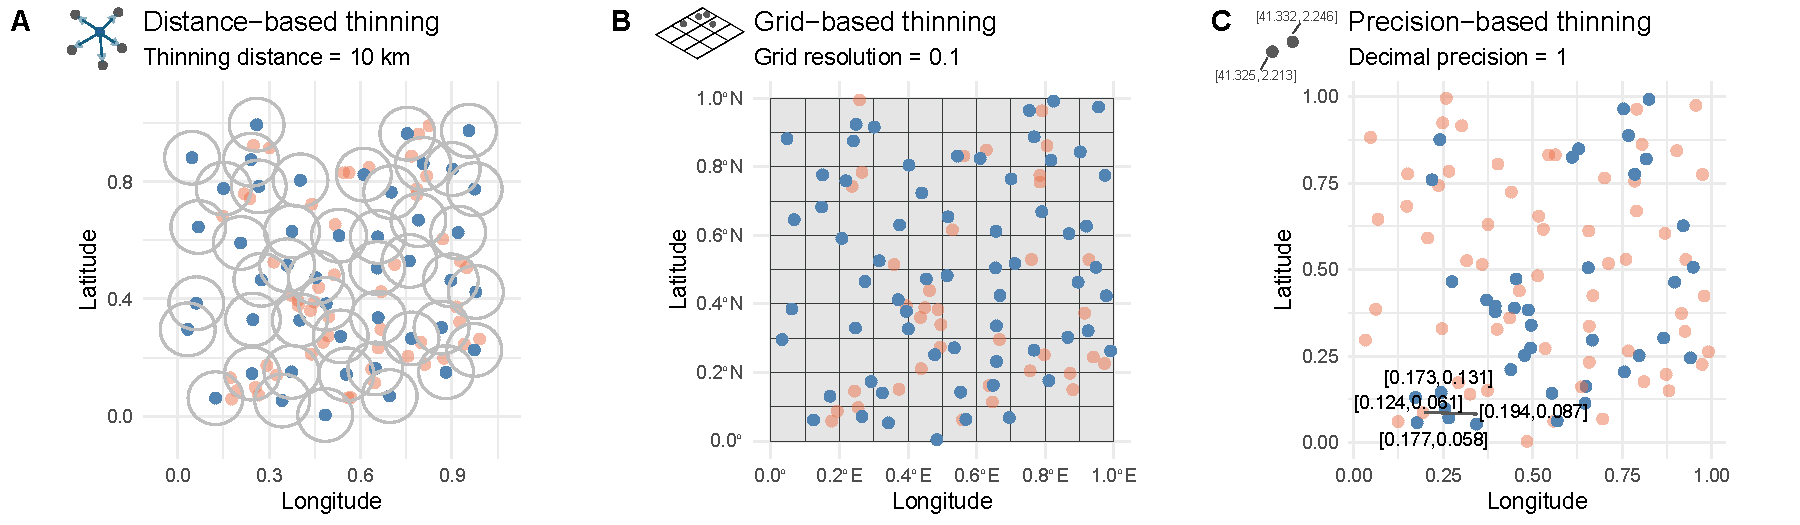
\includegraphics[width=1\linewidth,alt={Three subplots comparing distance-based, grid-based, and precision-based thinning. Each plot shows retained points in blue and removed points in red across a unit square.}]{figures/Figure_1_thin_methods} \caption{Spatial thinning examples using the three methods implemented in GeoThinneR: (A) distance-based thinning with a thinning distance of 10 km, (B) grid-based thinning with a grid resolution of 0.1 degrees and retaining one point per grid cell, and (C) precision-based thinning with coordinates rounded to one decimal place. Blue points indicate retained points and red points those removed during the thinning process.}\label{fig:thinmethods}
\end{figure}

The optimized algorithms described in the next section focus on distance-based thinning (\texttt{method\ =\ "distance"}), since the other methods do not rely on neighbour searches and have lower computational cost.

\subsection{Optimization for large datasets}\label{optimization-for-large-datasets}

As the size of spatial datasets increases, finding exact nearest neighbors by scanning the complete set \(\mathbf{S}\) and computing all pairwise distances for each query point \(q\) becomes computationally unfeasible. This makes nearest neighbor searches one of the primary bottlenecks in spatial thinning methods with exact distance thresholds. To address this, \CRANpkg{GeoThinneR} implements four different search strategies:

\begin{itemize}
\tightlist
\item
  \texttt{search\_type="brute"} is a greedy algorithm similar to the one implemented in \CRANpkg{spThin} and \CRANpkg{enmSdmX}, which calculates all pairwise distances between points using the \CRANpkg{fields} package \citep{fieldsRpackage}. While being the most straightforward approach, it scales poorly with large datasets due to its \(O(n^2)\) complexity.
\item
  \texttt{search\_type="kd\_tree"} uses \emph{kd}-tree structures from the \CRANpkg{nabor} package \citep{elsebergcomparison}, which were proposed to theoretically reduce nearest-neighbor searches time complexity to \(O(\log n)\) \citep{friedman1975algorithm}. Although \emph{kd}-trees can significantly improve performance for large datasets, they may suffer from the ``curse of dimensionality'' or in cases where exhaustive searches are required to identify exact nearest neighbors, their performance can be equivalent to or worse than brute-force algorithms \citep{ram2019revisiting}.
\item
  \texttt{search\_type="local\_kd\_tree"} subdivides the spatial domain into multiple subregions, each with an independent and smaller \emph{kd}-tree. This avoids creating a single large \emph{kd}-tree where lots of queries have to be evaluated and reduces both run time and memory usage for large datasets by building smaller and more manageable search trees.
\item
  \texttt{search\_type="k\_estimation"} is an alternative approach to improve \emph{kd}-tree performance and scalability. When searching for nearest-neighbors within a given distance, the exact number of neighbors \(k\) per query point \(q\) is unknown, so the algorithm evaluates whether all points in the tree lie within the search radius bound from \(q\). To reduce the number of searches performed in the tree for each query point \(q\), we propose a method to estimate the maximum possible number of neighbors \(k_\text{max}\). This estimation reduces the number of searches per point from \(n\) to \(k_\text{max}\), reducing unnecessary computations of distant points while still finding the exact number of neighbors.
\end{itemize}

These optimizations significantly improve computational efficiency, making \CRANpkg{GeoThinneR} suitable for large-scale SDM applications. The underlying algorithms and their performance trade-offs are further detailed in Section~\hyperref[modifiedthinning]{3}.

\subsection{Additional functionalities}\label{additional-functionalities}

In addition to its core thinning methods, \CRANpkg{GeoThinneR} includes several functionalities designed for SDM workflows that users may require when running their analysis. Firstly, \CRANpkg{GeoThinneR} allows performing group-specific thinning within a single dataset. This is useful when working with datasets containing multiple groups, such as different species or presence/absence data, where thinning needs to be applied independently within each group (Figure \ref{fig:addfeat}a).

\begin{verbatim}
# Thinning by group
precision_thin_group <- thin_points(sim_data,
  method = "precision", precision = 1,
  group_col = "group", seed = 2948
)
\end{verbatim}

Secondly, in some cases, users may need to retain a fixed number of points while maintaining spatial representativeness, such as for class balancing in presence/absence datasets. \CRANpkg{GeoThinneR} allows users to specify a target number of retained points and attempts to retain the specified number of points while guaranteeing a minimum distance threshold between them (Figure \ref{fig:addfeat}b). The process for retaining points selects the most spatially distant points to maximize geographical representativeness. This approach is supported only via the brute-force method as it requires all pairwise distance computations to select the most distant points.

\begin{verbatim}
# Thinning target points
target_thin <- thin_points(sim_data, target_points = 20, thin_dist = 10, seed = 675)
\end{verbatim}

Finally, when applying the thinning algorithm and deciding which points to remove and retain, users can specify variables that influence which points are preferentially retained, making it possible to prioritize records based on ecological relevance, data quality, or uncertainty (Figure \ref{fig:addfeat}c). The thinning algorithm follows the standard procedure, but when multiple candidate points violate the thinning constraint, such as falling within the same grid cell or minimum distance threshold, the algorithm retains the point with the highest priority value. This gives users more control over the characteristics of the retained dataset. For example, heterogeneous datasets from sources such as GBIF often include records of varying spatial precision. In such cases, prioritization allows users to preferentially retain higher-quality records instead of selecting points at random.

\begin{verbatim}
# Thinning priority
sim_data$priority <- runif(100, 1, 5)
rast_obj <- terra::rast(xmin = 0, xmax = 1, ymin = 0, ymax = 1, res = 0.2)
priority_thin <- thin_points(sim_data,
  method = "grid", raster_obj = rast_obj,
  priority = sim_data$priority, seed = 3455
)
\end{verbatim}

\begin{figure}
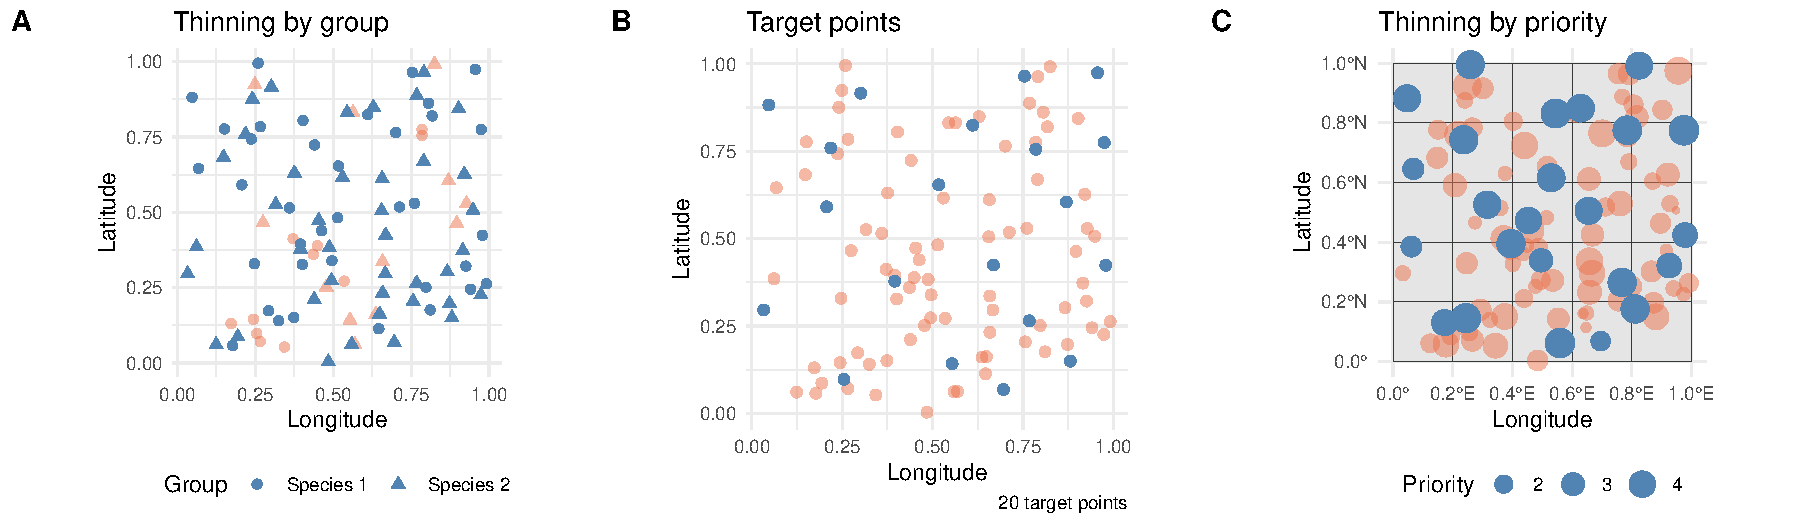
\includegraphics[width=1\linewidth,alt={Three subplots showing additional functionalities of GeoThinneR: group-wise thinning, retaining a fixed number of points, and pioritizing points based on larger variable values within each grid cell.}]{figures/Figure_2_add_feat} \caption{Additional spatial thinning functionalities available in GeoThinneR: (A) group-wise thinning applied independently for each species (B) retaining a fixed number of points (20 points in this example) while ensuring spatial separation, and (C) prioritizing points based on larger variable values within each grid cell. Retained points are shown in blue, and removed points are in red.}\label{fig:addfeat}
\end{figure}

\section{Modified distance-based thinning algorithm based on kd-tree}\label{modifiedthinning}

The distance-based thinning process can be conceptualized as a two-step procedure: (1) identifying neighboring points within a given distance threshold, and (2) selectively removing points to meet the selection criteria. Current methods in SDM workflows use greedy approaches in the first step, computing all pairwise distances between points and resulting in a time complexity of \(O(n^2)\) and high memory usage. \CRANpkg{GeoThinneR}, like \CRANpkg{spThin} \citep{aiello2015spthin} and \CRANpkg{enmSdmX} \citep{smith2023including}, implements a brute-force method using the \texttt{rdist.earth()} function from the \CRANpkg{fields} package \citep{fieldsRpackage}. To improve performance, we propose two minor modifications to \emph{kd}-tree nearest-neighbor search algorithms improving scalability for large datasets (Figure \ref{fig:distthinalg}). These methods reduce computational complexity while ensuring exact thinning distances, so they do not change which points are retained.

\begin{figure}
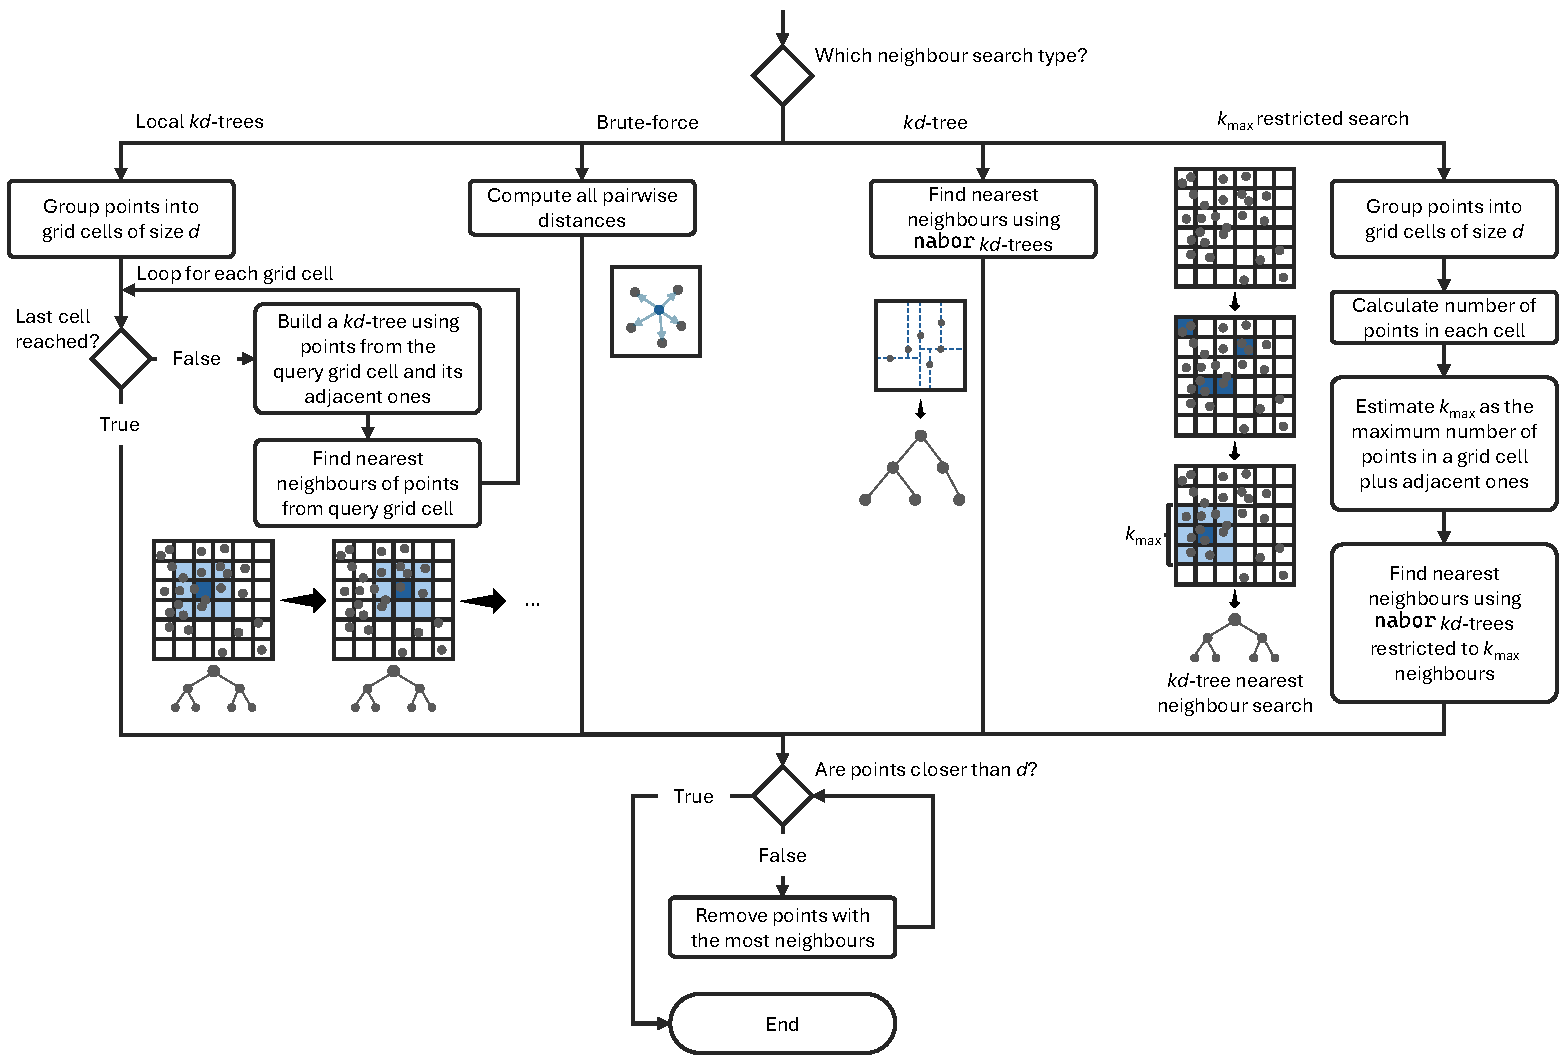
\includegraphics[width=1\linewidth,alt={Flowchart with four main branches representing the different search types for the distance-based thinning method implemented in GeoThinneR: local kd-trees, brute-force, standard kd-tree, and restricted kd-tree. Each path shows decision nodes, grids, and kd-tree icons ending in a shared loop for checking and removing neighbors.}]{figures/Figure_3_distance_thinning_algorithm} \caption{Diagram illustrating the four nearest neighbor search strategies implemented in GeoThinneR for distance-based thinning. The methods include brute-force, standard kd-trees, local kd-trees, and restricted kd-trees using estimated k-max. Each approach computes neighboring points within a thinning distance before proceeding with point removal.}\label{fig:distthinalg}
\end{figure}

\subsection{Traditional kd-tree nearest neighbor search}\label{traditional-kd-tree-nearest-neighbor-search}

A \emph{kd}-tree \citep{friedman1975algorithm} is a data structure that organizes points in a \(k\)-dimensional space by recursively partitioning the data along hyperplanes creating a binary search tree. Each node in the \(kd\)-tree represents a data point in the multidimensional space, and internal (non-leaf) nodes define the splitting hyperplanes that divide the space into two subsets of points based on their position relative to the split \citep{ram2019revisiting}. Many \emph{kd}-tree variants exist, but the essence is that they recursively partition the space containing the set of points \(\mathbf{S}\) into hyper-rectangles that contain a small subset \(\mathbf{S}'_i \subset \mathbf{S}\) of the input points \citep{panigrahy2008improved}.

\CRANpkg{GeoThinneR} implements \emph{kd}-tree construction and nearest-neighbor searches using the \CRANpkg{nabor} package, which wraps the \texttt{libnabo} library \citep{elsebergcomparison}. Since these \emph{kd}-trees are built on Euclidean distances, geographic coordinates (latitude and longitude) are transformed into Cartesian coordinates \((x, y, z)\) before constructing the binary tree:
\begin{equation}
\begin{split}
x &= R \cdot \cos(\text{lat}) \cdot \cos(\text{lon}) \\
y &= R \cdot \cos(\text{lat}) \cdot \sin(\text{lon}) \\
z &= R \cdot \sin(\text{lat}),
\end{split}
  \label{eq:cartesian}
\end{equation}
where \(\text{lat}\) and \(\text{lon}\) are the latitude and longitude in radians, respectively (\(\frac{\pi}{180}(\text{lon}, \text{lat})\)), and \(R\) is the Earth's radius. This results in a three-dimensional \emph{kd}-tree.

However, performance may be worsened in higher dimensions or when many points must be evaluated as potential neighbors of the query point \(q\). The time required to find the neighbors of \(q\) is affected by the search for candidate neighbors and the time it takes to evaluate among all candidates which ones are actually neighbors \citep{ram2019revisiting}. While approximate searches can reduce computational time by tuning the precision-recall trade-off, exact searches in large datasets require exhaustive searches, leading to higher computational complexity. To improve scalability, we introduce two additional optimizations: local \emph{kd}-trees partitioning and restricted neighbor searches.

\subsection{Local kd-trees for scalable searches}\label{local-kd-trees-for-scalable-searches}

To reduce the complexity of searching within a single \emph{kd}-tree constructed for the entire set of points \(\mathbf{S}\), which requires evaluating all points to identify neighbors within the distance threshold, we propose constructing local \emph{kd}-trees by subdividing the spatial domain into multiple smaller regions, each with its own tree. Although creating multiple \emph{kd}-trees is time-consuming, memory usage and overall runtime are improved for large datasets, as neighbor searches are less exhaustive when evaluating smaller subsets \(\mathbf{S}'_i \subset \mathbf{S}\).

To find exact neighbors using this approach, we first divide the spatial domain into a grid with cell sizes equal to the thinning distance and assign each point to a grid cell. Then, for each grid cell, we identify points within that cell and its adjacent cells, as these are potential neighbors. Recursively, an independent \emph{kd}-tree is constructed for each grid cell using the \CRANpkg{nabor} package, and neighbors are identified for each query point within the cell.

This strategy maintains computational efficiency while avoiding memory overloads of constructing and querying large trees. Furthermore, \CRANpkg{GeoThinneR} uses parallel processing when \texttt{n\_cores} is set to a value greater than one, providing a straightforward way to scale thinning operations across large datasets.

\subsection{Restricted neighbor searches}\label{restricted-neighbor-searches}

When performing the nearest-neighbor searches using \emph{kd}-trees from \CRANpkg{nabor}, we have to specify the number of neighbors to find \(k\) which increases or decreases the search complexity. As the number of potential neighbours for a point \(q\) is unknown, we set \(k\) equal to the total number of points \(n\) in the dataset, ensuring that all points are checked to determine whether they are neighbors of the query point. However, for large datasets, this approach introduces unnecessary computational costs by evaluating distant points. Instead, we propose an adaptive neighbor search that estimates \(k_{\text{max}}\) based on local point densities to reduce the number of nearest neighbors to find for each query point.

The process involves dividing the spatial domain into grid cells of size equal to the thinning distance \(d\), then counting the number of points in each grid cell and identifying the densest cells. The maximum number of neighbors a point may have \(k_{\text{max}}\) is estimated as the maximum number of points found within any dense cell and its adjacent cells. This value provides a practical upper bound on the neighbour search and is used to limit the number of points evaluated during the \emph{kd}-tree query, reducing unnecessary searches while still ensuring exact neighbour identification.

This method significantly reduces computational time, particularly in datasets where the maximum number of neighbors per point is much smaller than the total number of points. However, one limitation is that densely populated areas or large thinning distances may inflate \(k_{\text{max}}\), making the method less effective. In such cases, the local \emph{kd}-tree method with parallelization provides a suitable alternative.

\subsection{Performance comparison of neighbor search methods}\label{performancesearchtype}

In this section, we evaluate the computational efficiency of the different neighbor search methods implemented in \CRANpkg{GeoThinneR} using simulated datasets of varying sizes and spatial structures. All tests were conducted using R 4.3.3 on a Windows 11 computer with 128 GB of RAM and an Intel(R) Xeon(R) Gold 6240R processor featuring 24 cores, 48 threads, and a base clock speed of 2.40 GHz. The benchmark code is available in the supplementary R files.

We simulated datasets within a unit square domain \([0,1] \times [0,1]\), ranging from 1,000 to 50,000 points, under three spatial processes to mimic different real-world scenarios: (i) a homogeneous Poisson process simulating complete spatial randomly distributed points, (ii) a Matern clustered point process generated using the \texttt{rMatClust} function from the \CRANpkg{spatstat} package \citep{spatstatRpackage} with 10 cluster centers (\texttt{kappa}), a cluster radius of 0.15 (\texttt{scale}), and a varying number of points per cluster (\texttt{mu}), and (iii) a mixed spatial pattern dataset combining the randomly distributed points and the clustered processes. Finally, we benchmarked the methods using two thinning distances (1 km and 10 km) to highlight the impact of increasing the number of points that need to be removed and how each method scales with different search complexities.

We compared the neighbor search methods in \CRANpkg{GeoThinneR} using execution time (seconds) and peak RAM usage (MB) to evaluate the computational speed and memory requirements, which are critical for large-scale spatial datasets. Each method was tested three times, and the mean values were calculated.

The two modified algorithms (\(k_\text{max}\) estimation and local \emph{kd}-trees) consistently outperform the brute-force and traditional \emph{kd}-tree methods in both peak memory usage (Figure \ref{fig:benchmarksearchtype}a) and execution time (Figure \ref{fig:benchmarksearchtype}b) across all spatial data types. The traditional \emph{kd}-tree method provides better performance compared to the brute-force method for small datasets; however, for larger datasets, memory usage and execution time increase due to exhaustive searches in deeper trees to find all neighbors of each point. However, the two optimized methods are orders of magnitude faster and less memory-intensive. For small thinning distances, the \(k_\text{max}\) estimation algorithm shows the best performance in terms of both time and memory usage, because the estimated number of neighbors \(k_\text{max}\) remains low, reducing unnecessary searches. However, at larger thinning distances, and particularly for the clustered and mix datasets, as the dataset size increases, this algorithm goes slower and uses more memory than the local \emph{kd}-trees approach. This is because the algorithm estimates a high value for \(k_\text{max}\) and, therefore, increases search complexity.

Alternatively, the local \emph{kd}-tree approach, which generates an independent \emph{kd}-tree for each subregion, offers improved memory efficiency and outperforms the other methods as thinning distances increase, as fewer trees need to be built. This method can also be executed in parallel, which can further improve run time for large datasets, especially when many partitions are created due to a small thinning distance or a large spatial extent (Figure \ref{fig:benchmarksearchtype}c). However, if the number of partitions is not very large, as in the case of the 1 km thinning distance in this example, parallel execution may not bring any improvement.

\begin{figure}
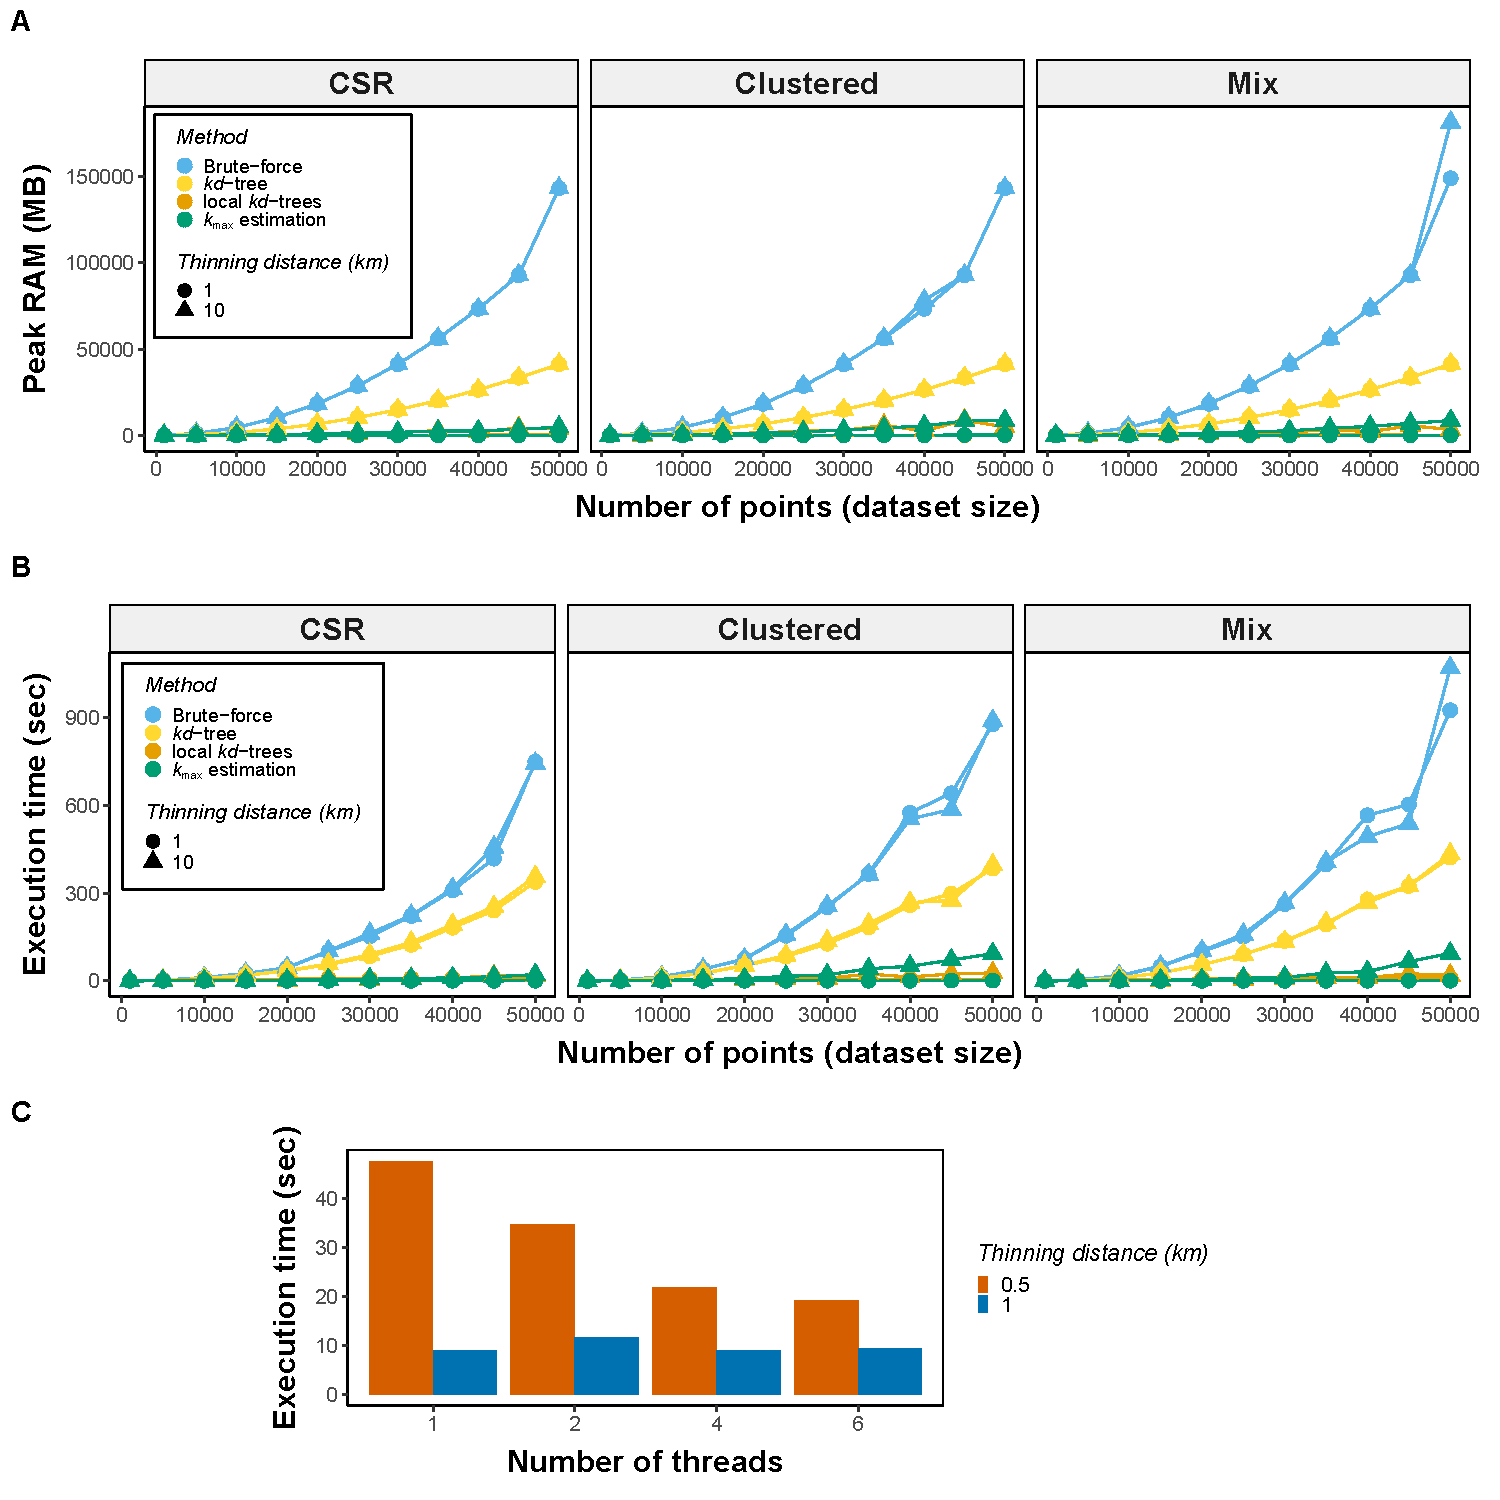
\includegraphics[width=1\linewidth,alt={Lineplots showing the benchmark results of neighbor search strategies in GeoThinneR. The plots compare execution time and memory usage across data types and methods.}]{figures/Figure_4_benchmark_search_type} \caption{Performance benchmark for neighbor searches implemented in GeoThinneR distance-based thinning. (A) Peak RAM usage (MB) and (B) execution time (seconds) across three spatial data types (CSR, clustered, and mixed spatial pattern) for dataset sizes ranging from 1,000 to 50,000 points. (C) Performance comparison of local kd-trees with parallelization for 50,000 randomly distributed points using two thinning distances (0.5 km and 1 km). The optimized algorithms (local kd-trees and k-estimation) scale better and provide superior computational efficiency than brute-force and standard kd-tree, especially for large datasets.}\label{fig:benchmarksearchtype}
\end{figure}

\section{Performance benchmark}\label{performancethinning}

In this section, we compare the performance of \CRANpkg{GeoThinneR} with two widely used R packages for spatial thinning: \CRANpkg{spThin} and \CRANpkg{enmSdmX}. We compare the execution time and memory usage of the distance-based thinning algorithms available in \CRANpkg{GeoThinneR} version 2.0.0 against the \texttt{thin()} function from \CRANpkg{spThin} version 0.2.0 and the \texttt{geoThin()} function from \CRANpkg{enmSdmX} version 1.2.10. In Section~\hyperref[benchsim]{4.1}, we compare the performance using simulated data, and in Section~\hyperref[benchreal]{4.2}, we benchmark the methods using a real-world large dataset.

\begin{verbatim}
brute <- thin_points(data,
  method = "distance", search_type = "brute",
  thin_dist = thin_dist, trials = trials
)
kd_tree <- thin_points(data,
  method = "distance", search_type = "kd_tree",
  thin_dist = thin_dist, trials = trials
)
local_kd_tree <- thin_points(data,
  method = "distance", search_type = "local_kd_tree",
  thin_dist = thin_dist, trials = trials
)
k_estimation <- thin_points(data,
  method = "distance", search_type = "k_estimation",
  thin_dist = thin_dist, trials = trials
)
spThin <- thin(data,
  lat.col = "lat", long.col = "lon", spec.col = "group",
  thin.par = thin_dist, reps = trials, locs.thinned.list.return = TRUE,
  write.files = FALSE, write.log.file = FALSE, verbose = FALSE
)
enmSdmX <- geoThin(data, 
  minDist = thin_dist * 1000, longLat = c("lon", "lat"), method = "complete"
)
\end{verbatim}

\subsection{Benchmark with simulated data}\label{benchsim}

The benchmark tests were performed on the complete thinning workflow using the simulated datasets described in Section~\hyperref[performancesearchtype]{3.4}. Each thinning method was executed with a single trial to obtain the maximum number of retained points per run, and each test was repeated three times to ensure reliable timing estimates. Here, we compared all methods across three spatial data types (random, clustered, and mixed) using again two thinning distances of 1 and 10 kilometers.

The optimized algorithms implemented in \CRANpkg{GeoThinneR} demonstrate significant improvements in both memory efficiency (Figure \ref{fig:benchmarkthinning}a) and execution time (Figure \ref{fig:benchmarkthinning}b) compared to existing tools. The \CRANpkg{enmSdmX} package exhibited the longest execution times, making it unsuitable for large datasets, so we limited its tests to 20,000 points. \CRANpkg{spThin}, although it's more efficient, shows similar performance to the brute-force method from \CRANpkg{GeoThinneR}. In contrast, our new modified methods demonstrate better scalability in both runtime and peak memory usage, making them more practical for large-scale spatial thinning.

The local \emph{kd}-tree and \(k_\text{max}\) estimation algorithms in \CRANpkg{GeoThinneR} present the best scalability for large datasets. Patterns are similar to the ones when comparing the neighbor search methods. The \(k_\text{max}\) estimation method is best suited for small thinning distances and without relatively dense regions, while the local \emph{kd}-tree method offers a good alternative for highly clustered datasets or large thinning distances. This flexibility ensures that \CRANpkg{GeoThinneR} can adapt to various real-world SDM workflows more efficiently than existing tools

\begin{figure}
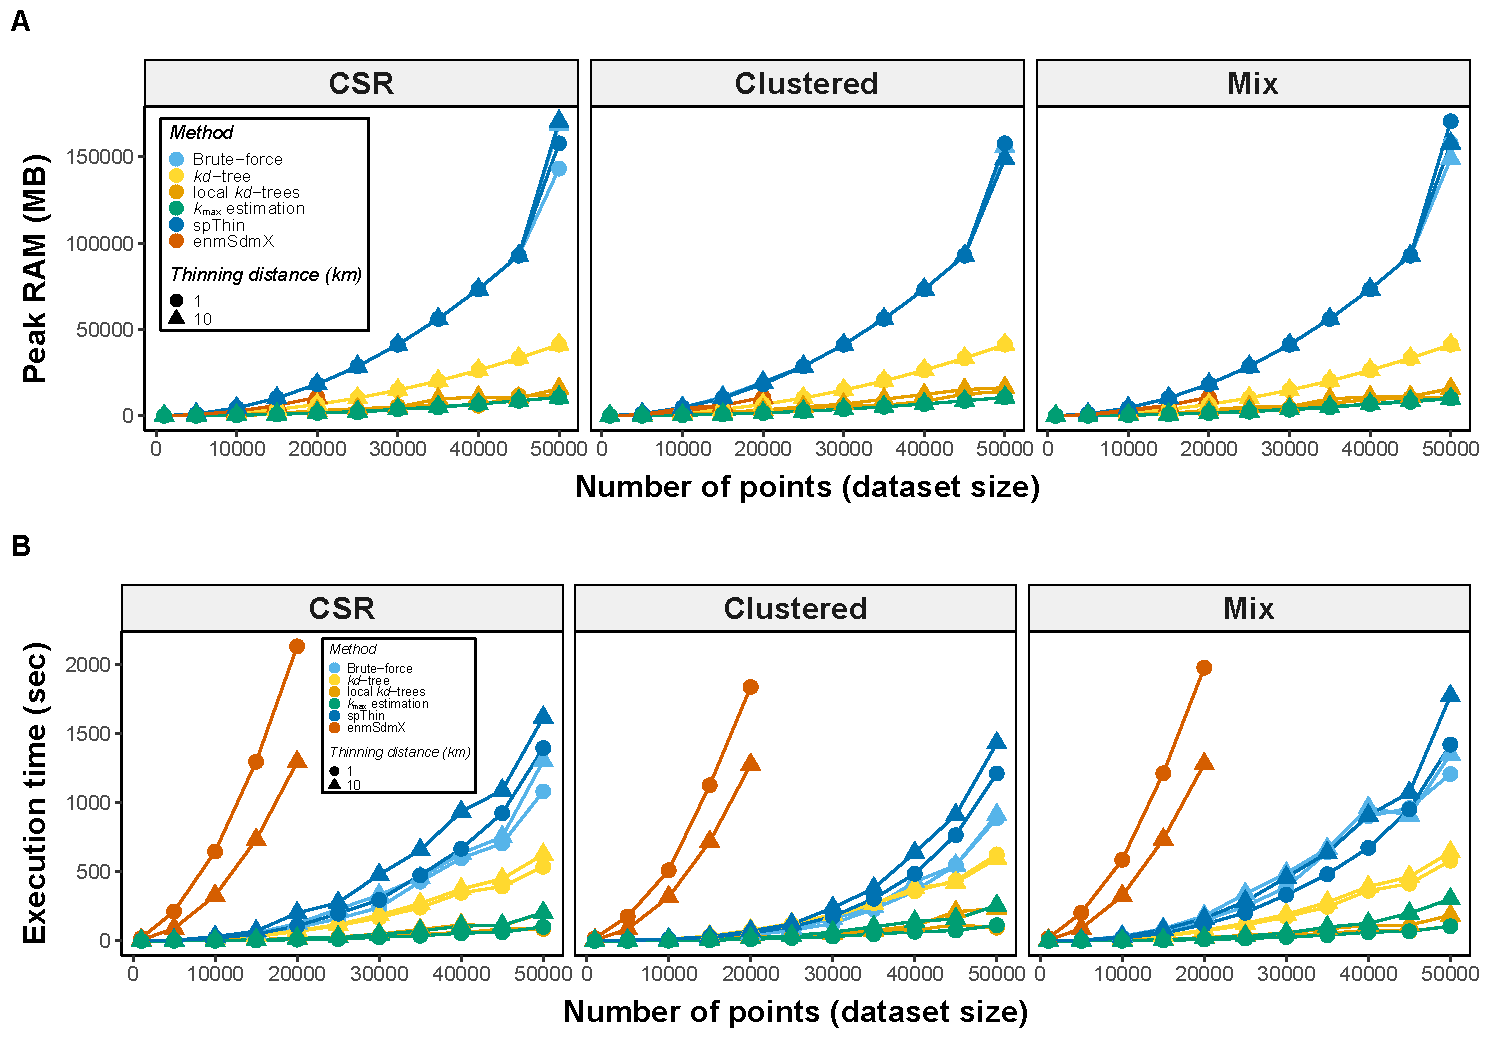
\includegraphics[width=1\linewidth,alt={Two panels showing line plots for peak RAM usage and execution time for three spatial thinning packages (GeoThinneR, spThin, enmSdmX) across three types of spatial point patterns and increasing dataset sizes. The enmSdmX curves stop earlier due to computational limits.}]{figures/Figure_5_benchmark_thinning} \caption{Performance benchmark for distance-based thinning across GeoThinneR, spThin, and enmSdmX. (A) Peak RAM usage (MB) and (B) execution time (seconds) across three spatial data types for varying dataset sizes. The enmSdmX method was only evaluated up to 20,000 points due to its high computational cost on larger datasets. The optimized methods of GeoThinneR (local kd-trees and k-estimation) offer better memory and runtime performance across all settings.}\label{fig:benchmarkthinning}
\end{figure}

\subsection{Application to real-world data}\label{benchreal}

To illustrate the performance of \CRANpkg{GeoThinneR} on real-world datasets, we applied its optimized thinning methods and compared them with \CRANpkg{spThin}. We used a small dataset of 8,340 occurrence records for the loggerhead sea turtle (\emph{Caretta caretta}) in the Mediterranean Sea \citep{GBIFCaretta}, and a large and highly clustered dataset of 80,163 points for the yellowfin tuna (\emph{Thunnus albacares}) collected globally from 1950 to 2025 \citep{GBIFThunnus}. Both datasets were downloaded from GBIF \citep{GBIF} and are very heterogeneous including data from different sources, locations, and sampling methods. The data are available in \CRANpkg{GeoThinneR} package and can be loaded using the \texttt{data()} function.

\begin{verbatim}
# Loggerhead sea turtle
data(caretta)
# Yellowfin tuna
data(thunnus)
\end{verbatim}

Here we show the performance of the local \emph{kd}-tree and \(k_\text{max}\) estimation algorithms implemented in \CRANpkg{GeoThinneR}, comparing their computational performance against \CRANpkg{spThin} using varying thinning distances. The objective is to show the trade-offs, best- and worst-case scenarios for each method, that's why we use varying thinning distances and dataset sizes. So we are not trying to identify the optimal thinning distance for SDM applications, this comparison highlights the scalability and efficiency of the algorithms. It is important to note that choosing an appropriate thinning distance for SDM is challenging and often requires being tuned empirically \citep{veloz2009spatially, soley2019sufficient}.

The results, shown in Figure \ref{fig:benchmarkrealdata}, show significant performance differences even for the smaller dataset. \CRANpkg{GeoThinneR} not only executed faster but also demonstrated substantially lower memory usage, addressing one of the key limitations of current spatial thinning methods in SDM (Figure \ref{fig:benchmarkrealdata}a). The \(k_\text{max}\) estimation algorithm was particularly efficient, with run times between one and two seconds due to low neighbor density that minimizes search complexity.

In contrast, the yellowfin tuna large dataset presented a different scenario (Figure \ref{fig:benchmarkrealdata}b). \CRANpkg{spThin} failed to execute due to excessive memory demands, surpassing our 128 GB RAM limit after several minutes, which highlights the scalability challenges of brute-force methods. Both algorithms in \CRANpkg{GeoThinneR} maintained low memory usage, even at this dataset size. However, the \(k_\text{max}\) estimation method experienced slower performance as thinning distances increased because the dataset presents highly clustered ares which inflate \(k_\text{max}\) estimates and increase search complexity. To address this, the local \emph{kd}-tree approach, executed here with multithreading (6 threads), proved both faster and less memory-intensive, being the method with best performance in this context. These results illustrate that while \(k_\text{max}\) estimation is highly efficient for moderately sized or uniformly distributed datasets, the local \emph{kd}-tree method with parallelization offers a memory-efficient solution for large and dense datasets.

\begin{figure}
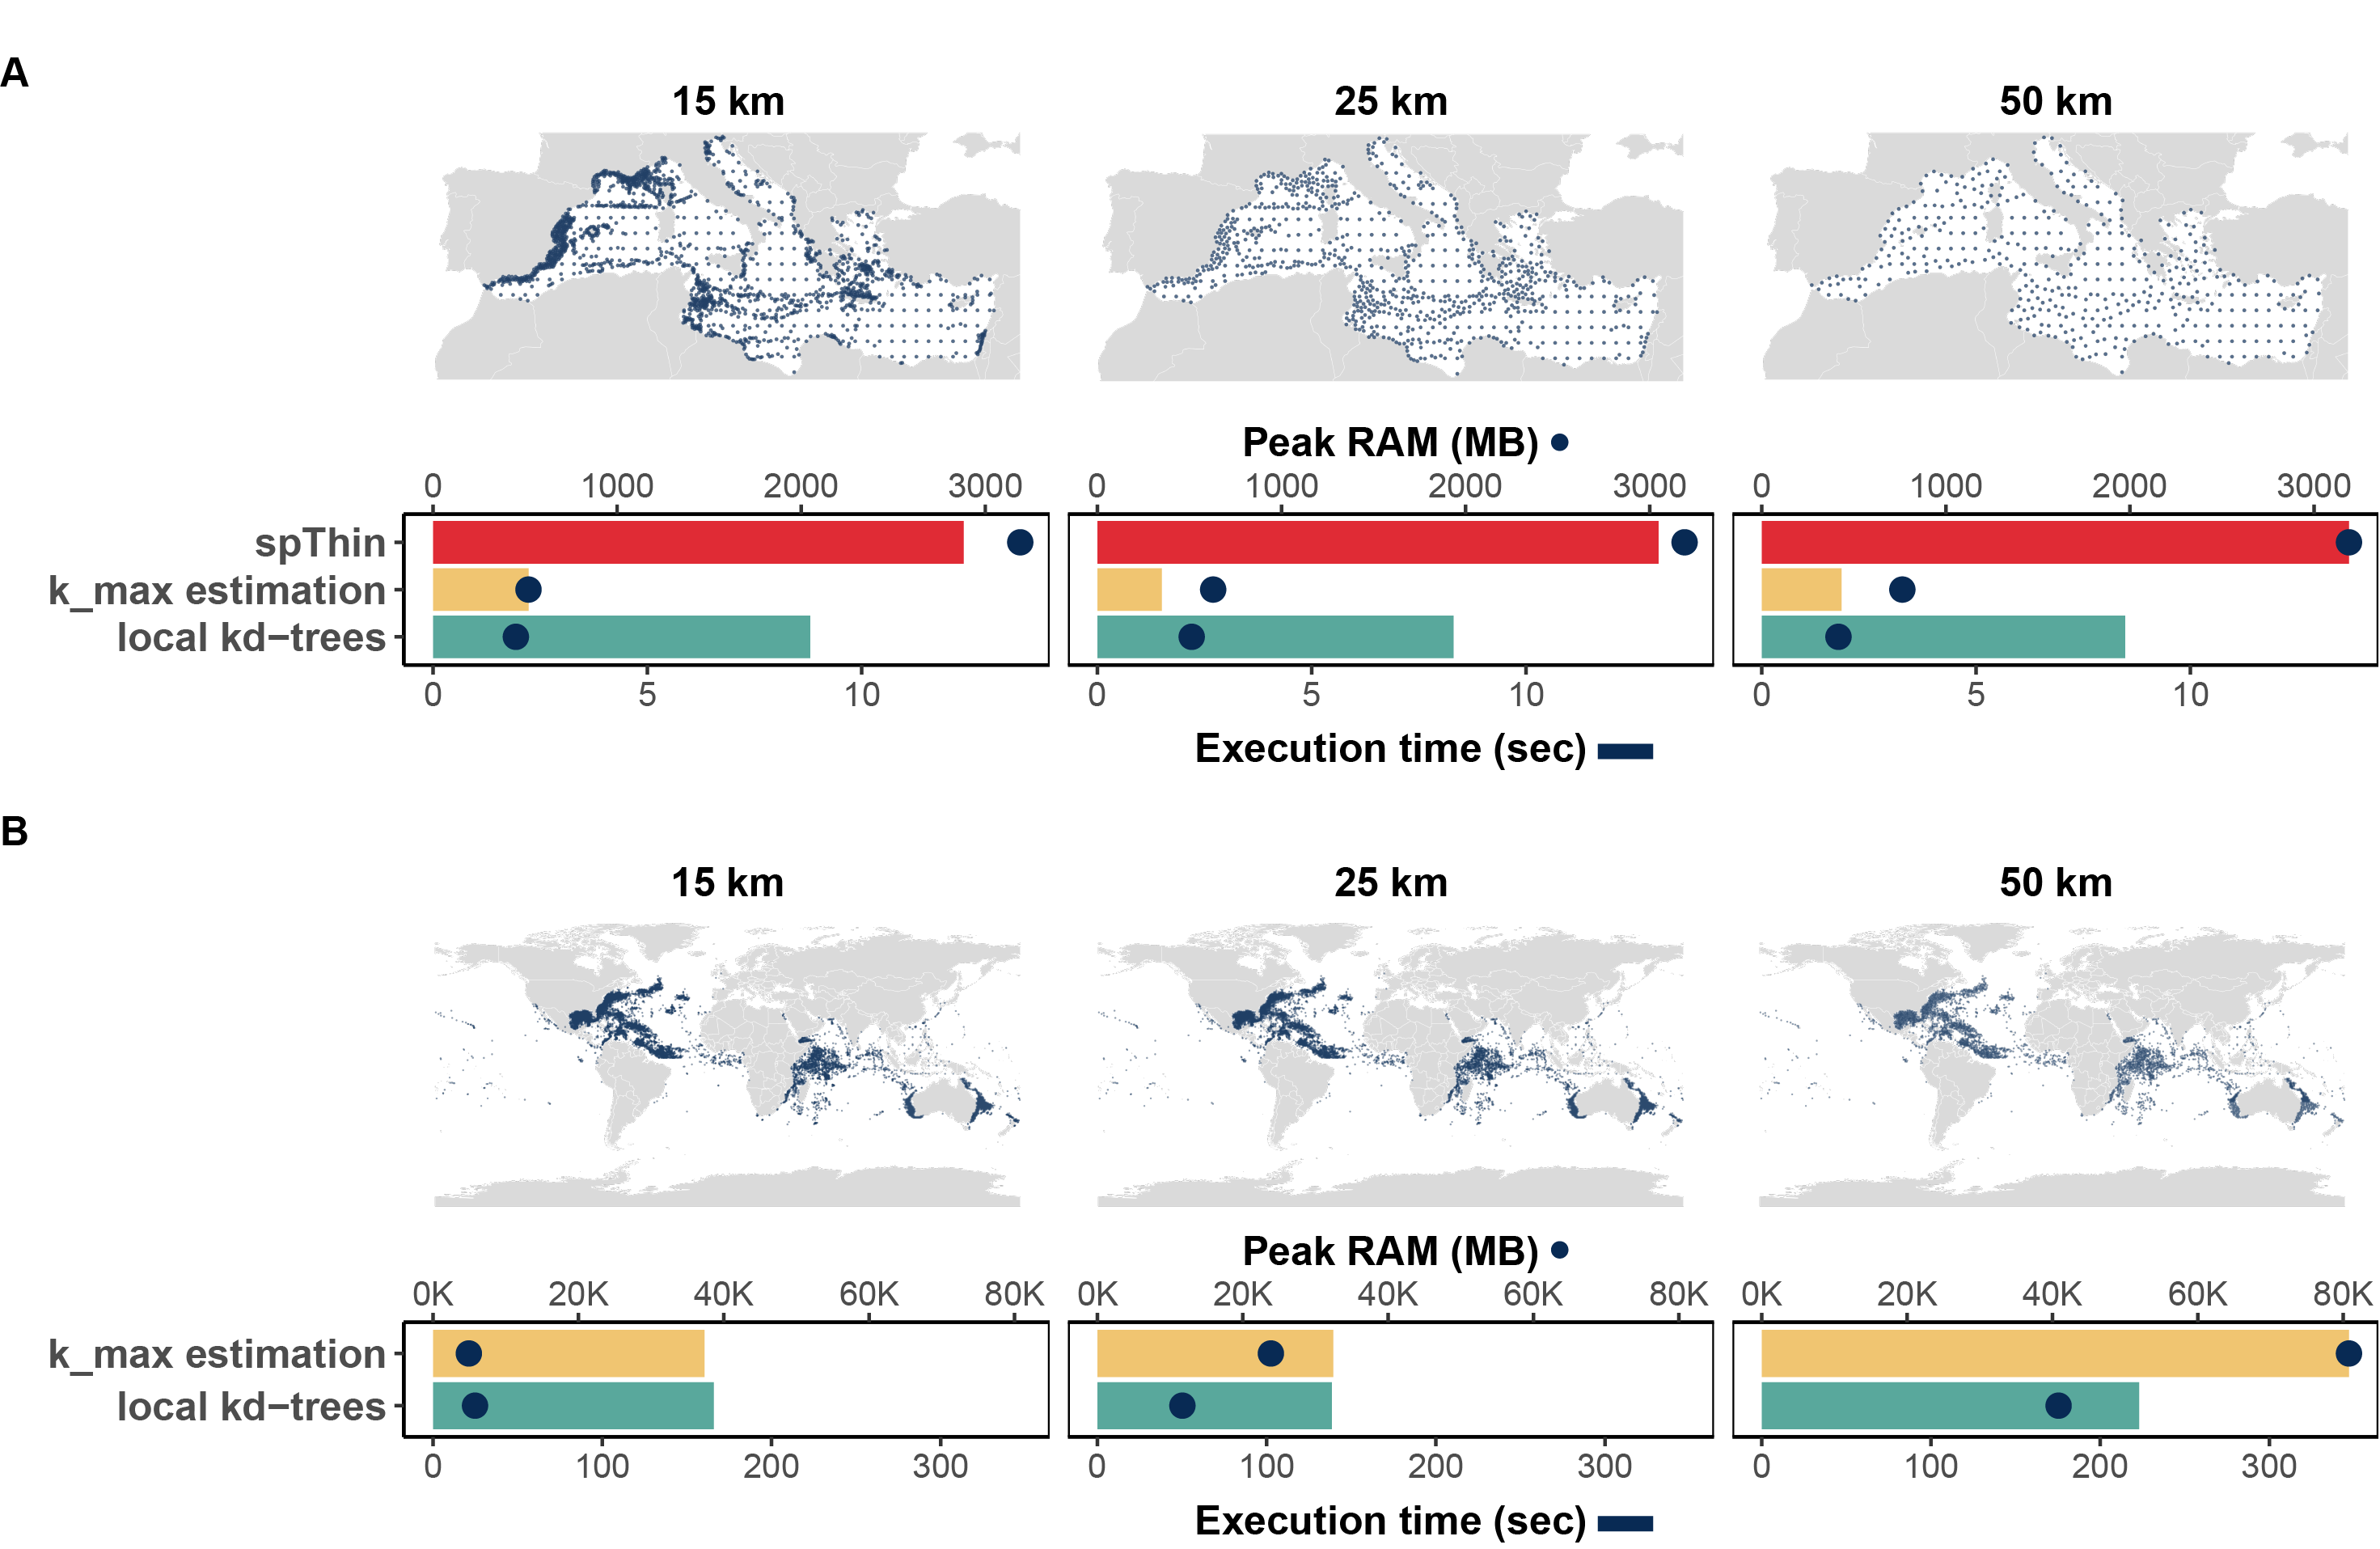
\includegraphics[width=1\linewidth,alt={Two panels comparing spatial thinning performance using bar plots and point symbols. Panel A shows thinned locations of loggerhead turtles in the Mediterranean and associated memory/time usage for the three methods. Panel B shows global thinning of yellowfin tuna records, with bars for execution time and points for memory usage for the two GeoThinneR methods only.}]{figures/Figure_6_benchmark_real} \caption{Execution time (bars) and memory usage (points) of GeoThinneR and spThin across varying thinning distances for occurrence data of (A) loggerhead turtles and (B) yellowfin tuna from GBIF. For the yellowfin tuna dataset, the results for spThin are not shown because the run could not be completed due to excessive memory usage.}\label{fig:benchmarkrealdata}
\end{figure}

Here we present the code used to generate the thinned datasets represented in Figure \ref{fig:benchmarkrealdata}:

\begin{verbatim}
caretta_thin <- thin_points(
  caretta,
  lon_col = "decimalLongitude",
  lat_col = "decimalLatitude",
  method = "distance",
  thin_dist = thin_dist, # One of 10, 25, 50
  search_type = "k_estimation",
  trials = 10
)

thunnus_thin <- thin_points(
  thunnus,
  lon_col = "decimalLongitude",
  lat_col = "decimalLatitude",
  method = "distance",
  thin_dist = thin_dist, # One of 10, 25, 50
  search_type = "local_kd_tree",
  trials = 1,
  n_cores = 6
)
\end{verbatim}

\section{Conclusions}\label{conclusions}

The \CRANpkg{GeoThinneR} R package offers a flexible and scalable implementation of spatial thinning methods, addressing key limitations of existing tools. It integrates multiple thinning approaches (distance-, grid-, and precision-based) into a single wrapper function, enhancing usability. Also, by incorporating optimized \emph{kd}-tree algorithms for distance-based thinning, such as local \emph{kd}-tree partitioning and adaptive \(k_\text{max}\) estimation, the package significantly reduces execution time and memory usage for large datasets. Additionally, \CRANpkg{GeoThinneR} includes customization features designed for species distribution modeling workflows, such as group-wise thinning and point prioritization. While future developments should be made in improving the computational performance of distance-based methods, incorporating additional thinning approaches, and estimating an optimal thinning distance, \CRANpkg{GeoThinneR} represents a step forward in improving the efficiency of spatial thinning methods in SDM.

\section{Acknowledgments}\label{acknowledgments}

This package has been developed as part of the ProOceans (PID2020-118097RB-I00) and SOSPen (PID2021-124831OA-I00) projects funded by the Spanish Ministry of Science and Innovation. The author also acknowledges the support from the MOIRAI project (grant agreement no. 101180994) funded by the European Union under the Horizon Europe program. This work acknowledges the institutional support of the ``Severo Ochoa Center of Excellence'' accreditation (CEX2024-001494-S funded by AEI 10.13039/501100011033) to the Institute of Marine Science (ICM-CSIC). Additionally, this work is part of the Integrated Marine Ecosystem Assessments (iMARES) research group, funded by the Agència de Gestió d'Ajuts Universitaris i de Recerca of the Generalitat de Catalunya (2021 SGR 00435).

\section{Supplementary materials}\label{supplementary-materials}

Supplementary materials are available in addition to this article:

\begin{itemize}
\tightlist
\item
  \emph{GeoThinneR\_replication\_small.R}: reproduces examples and figures from Sections 2 and 3. Includes a short benchmark and demonstrations of package features using small datasets.
\item
  \emph{GeoThinneR\_replication\_large.R}: reproduces figures and results from Section 4. Includes a larger benchmark to evaluate performance of GeoThinneR and other packages using simulated and real-world datasets.
\item
  \emph{caretta\_download.R}: downloads occurrence data for loggerhead turtles (\emph{Caretta caretta}) from GBIF.
\item
  \emph{thunnus\_download.R}: downloads occurrence data for yellowfin tuna (\emph{Thunnus albacares}) from GBIF.
\item
  \emph{data/}: contains benchmark results and the cleaned loggerhead turtle and yellowfin tuna datasets used.
\end{itemize}

\bibliography{MestreTomas2026RJournalGeoThinneR.bib}

\address{%
Jorge Mestre-Tomás\\
Institut de Ciències del Mar (ICM-CSIC)Universitat Politècnica de València (UPV)\\%
Renewable Marine Resources Department, Barcelona, Spain\\ Department of Applied Statistics and Operational Research, and Quality, Valencia, Spain\\
%
\url{https://github.com/jmestret}\\%
\textit{ORCiD: \href{https://orcid.org/0000-0002-8983-3417}{0000-0002-8983-3417}}\\%
\href{mailto:jorgemestre@icm.csic.es}{\nolinkurl{jorgemestre@icm.csic.es}}%
}
